\documentclass[prb,12pt]{revtex4-2}
%fonts
% Palatino for main text and math
\usepackage[osf,sc]{mathpazo}

% Helvetica for sans serif
% (scaled to match size of Palatino)
\usepackage[scaled=0.90]{helvet}

% Bera Mono for monospaced
% (scaled to match size of Palatino)
\usepackage[scaled=0.85]{beramono}
\usepackage{amsmath, amssymb,physics,amsfonts,amsthm}
\usepackage{enumitem}
\usepackage{cancel}
\usepackage[most]{tcolorbox}
\usepackage{booktabs}
\usepackage{tikz}
\usepackage{hyperref}
\usepackage{enumitem}
\usepackage{transparent}
\usepackage{float}
\usepackage{multirow}
\usepackage{slashed}
\newtheorem{Theorem}{Theorem}
\newtheorem{Proposition}{Proposition}
\newtheorem{Lemma}[Theorem]{Lemma}
\newtheorem{Corollary}[Theorem]{Corollary}
\newtheorem{Example}[Theorem]{Example}
\newtheorem{Remark}[Theorem]{Remark}
\theoremstyle{definition}
\newtheorem{Problem}{Problem}
\theoremstyle{definition}
\newtheorem{Definition}[Theorem]{Definition}
\newenvironment{parts}{\begin{enumerate}[label=(\alph*)]}{\end{enumerate}}
\newcommand{\backvec}[1]{\reflectbox{$\vec{\reflectbox{\!$#1$}}$}}

%tikz
\usetikzlibrary{patterns}
\usepackage{tikz-cd}
% definitions of number sets
\newcommand{\N}{\mathbb{N}}
\newcommand{\R}{\mathbb{R}}
\newcommand{\Z}{\mathbb{Z}}
\newcommand{\Q}{\mathbb{Q}}
\newcommand{\C}{\mathbb{C}}
\allowdisplaybreaks

\newtcolorbox{revision}[1][]{empty, breakable, sharp corners, borderline north={1pt}{0pt}{black},
	borderline west={5pt}{0pt}{black},
	#1}

\begin{document}
	\title{Theory and Phenomenology of Superconductivity Homework 3}
	\author{Jun Wei Tan}
	\email{jun-wei.tan@stud-mail.uni-wuerzburg.de}
	\affiliation{Julius-Maximilians-Universit\"{a}t W\"{u}rzburg}
	\date{\today}
	\maketitle
%\begin{Problem}
	\begin{parts}
		\item Geben Sie die Definitionen von Gradient, Rotation und Divergenz an.
		\item Wir schreiben die Komponenten des dreidimensionalen Vektorprodukts als
			\[
				(\vec{a}\times \vec{b})_i=\sum_{j,k=1}^3 \epsilon_{ijk}a_jb_k,\] 
				wobei $\epsilon_{ijk}$ der total antisymmetrische Tensor f\"{u}r $\R^3$ ist, mit $\epsilon_{ijk}=1$. Zeigen Sie, dass gilt:
				\begin{align*}
					\sum_{i=1}^3 \epsilon_{ijk}\epsilon_{ilm}=&\delta_{jl}\delta_{km}-\delta_{jm}\delta_{kl}\\
					\frac{1}{2}\sum_{i,j=1}^3 \epsilon_{ijk}\epsilon_{jl}\delta_{kl},
				\end{align*}
				mit $\delta$ dem Kronecker-$\delta$.
			\item Zeigen Sie mit den Formeln aus (b) die folgenden Identitäten für beliebige Vektorfelder $\vec{a},~\vec{b},~\vec{c},~\vec{d}$:
				\begin{align*}
					\vec{a}\cdot(\vec{b}\times\vec{c})&=\vec{b}\cdot (\vec{c}\times \vec{a})=\vec{c}\cdot (\vec{a}\times \vec{b})\\
					\vec{a}\times(\vec{b}\times\vec{c})=&(\vec{a}\cdot\vec{c})\vec{b}-(\vec{a}\cdot\vec{b})\vec{c},\\
					(\vec{a}\times\vec{b})\cdot(\vec{c}\times\vec{d})=*(\vec{a}\cdot\vec{c})(\vec{b}\cdot\vec{d})-(\vec{a}\cdot\vec{d})(\vec{b}\cdot\vec{c})
				\end{align*}
			\item Zeigen Sie damit, dass f\"{u}r beliebige skalare Funktionen $F(\vec{x})$ und Vektorfelder $\vec{A}(\vec{x})$ gilt:
				\begin{align*}
					\curl{\grad{F}}=&0\\
					\div{(\curl{A})}=&0\\
					\curl{\curl{A}}=&\grad{(\div{A})}-\laplacian{A}\\
					\div{(F\vec{A})}=(\grad{F})\cdot\vec{A}+F\div{\vec{A}},
				\end{align*}
				mit $\Delta$ dem Laplace-Operator.
	\end{parts}
\end{Problem} 
\begin{proof}
	\begin{parts}
	\item 
		\begin{align*}
			\text{grad }F=\sum_{i=1}^3 \pdv{F}{x_i}\hat{x}_i\\
			\text{div }\vec{F}=\sum_{i=1}^3 \pdv{F_i}{x_i}\\
			\text{curl }\vec{F}=&\ldots
		\end{align*}
	\item Offensichtlich muss $j\neq k$ und $l\neq m$ sein, ansonsten wäre 1
	\end{parts}
\end{proof}
\begin{Problem}
	
\end{Problem}

%\begin{Problem}
	Betrachten Sie die folgenden Familien von Kraftfeldern auf geeigneten Definitionsbereichen $D_\eta^{(n)}  \subseteq \R^3$
	\begin{align*}
		F_\eta^{(1)}:& D_\eta^{(1)}\ni \va x\to r^\eta\cdot \va x\in \R^3\\
		F_\eta^{(2)}:& D_\eta^{(2)}\ni\va x \to r_{12}^\eta\cdot(x_1\va e_1-x_2\va e_2)\in \R^3\\
		F_\eta^{(3)}:& D_\eta^{(3)}\ni \va x\to r_{12}^\eta\cdot\left( x_2\va e_1-x_1\va e_2 \right) \in\R^3\\
		F_\eta^{(4)}:&D_\eta^{(3)}\ni \va x\to r_{12}^\eta\cdot\left( x_2\va e_1+x_1\va e_2 \right) \in \R^3
	\end{align*}
	wobei $r_{12}=\sqrt{x_1^2+x_2^2} $ und $r=\sqrt{x_1^2+x_2^2+x_3^3} $
	Skizzieren Sie die Felder $\va F_\eta^{(n)}$ als Vektorpfeile in der von den Einheitsvektoren $\va e_1$ und $\va e_2$ aufgespannten Ebene (hier genügt es, zwischen den Fällen $\eta > -1, \eta = -1$ und $\eta < -1$ zu unterscheiden). 
	
	Bestimmen Sie, abhängig von der Potenz $\eta \in \R$,
	\begin{enumerate}
		\item den maximalen Definitionsbereich $D_\eta^{(n)}$,
		\item die maximale Bereiche $C_\eta^{(n)}\subseteq D_\eta^{(n)}$, auf denen $F_\eta^{(n)}$ konservativ ist,
		\item eine Potentialfunktion $V_\eta^{(n)}:C_{\eta}^{(n)}\to \R$ mit $F_\eta^{(n)}=-\grad{V_\eta^{(n)}}$, sofern sie existiert,
		\item das Kurvenintegral
		\[I_\eta^{(n)}(R)=\int_{\gamma_R}\dd{\va\xi}\cdot\va F_\eta^{(n)}(\va\xi)\]
		über den gegen den Uhrzeigersinn umlaufenen Kreis $\gamma_R$ mit Radius $R$ und Mittelpunkt $\va0$ in der von $\va e_1$ und $\va e_2$ aufgespannten Ebene
		\begin{center}
			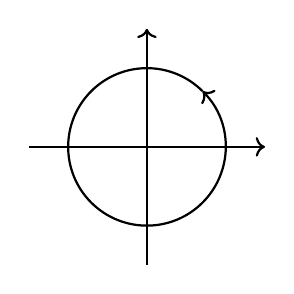
\begin{tikzpicture}
				\draw[thick, ->] (-1.5,0) -- (1.5,0);
				\draw[thick, ->] (0,-1.5) -- (0,1.5);
				\draw[thick, ->] ({1/sqrt(2)},{1/sqrt(2)}) arc (45:405:1);
			\end{tikzpicture}
		\end{center}
	\end{enumerate}
\end{Problem}

\begin{Problem}
	Let $V$ be a $\mathbb{K}$-valued vector space. A seminorm on $V$ is a homogeneous map $p:V\to [0,\infty)$ satisfying the triangle inequality, i.e.
	\[
	p(v+w)\le p(v)+p(w)
\]
and
\[
p(\lambda v)=|\lambda|p(v)
\]
for any two vectors $v,w\in V$ and every scalar $\lambda\in\mathbb{K}$.
\begin{parts}
	\item Show that the kernel of a seminorm $p$ is a subspace of $V$.

		Given a seminorm $p$, we say that two vectors $v,w\in V$ are equivalent if there is a vector $u\in \text{ker }p$ such that $w=v+u$. Make yourself clear that this yields an equivalence relation on $V$.
	\item Show that the quotient space $V / \text{ker }p:=V / \sim$ carries a canonical linear structure.
	\item Show that the map
		\[
			\overline{p}:V / \text{ker }p\ni [v]\mapsto p(v)
		\]
		yields a well-defined norm on the quotient space.
\end{parts}
\end{Problem}
\begin{proof}
	\begin{parts}
	\item Clear by definition
	\item Also clear
	\end{parts}
\end{proof}
\begin{Problem}\label{pr:funcanalblatt3-2}
	Let $M$ be a topological space. Show that the space $(\mathcal{C}_b(M), \|\cdot\|_\infty)$ of continuous and bounded $\mathbb{K}$-valued functions endowed with the supremum norm is complete.
\end{Problem}

\begin{Problem}
	In this exercise we weaken the conditions of Homework~\ref{pr:funcanalblatt3-2} by considering functions that are only essentially bounded. The goal is to find a suitable seminorm on this function space such that the corresponding quotient becomes a Banach space. But first, we shall settle the term ``essentially bounded''. To this end, we need the following definitions:

	Let $X$ be a set and $\mathfrak{a}\in 2^X$. We call $\mathfrak{a}$ a $\sigma$-algebra if
	\begin{itemize}
		\item $\varnothing\in\mathfrak{n}$,
		\item $X \setminus A\in \mathfrak{a}$ for every $A\in \mathfrak{a}$ and
		\item $\bigcup_{n\in \N} A_n\in \mathfrak{a}$ for every sequence $(A_n)_{n\in \N}\subset \mathfrak{a}$
	\end{itemize}
	The pair $(X, \mathfrak{a})$ is called a measurable space. One can check that for every $A\in \mathfrak{a}$ one obtains a new $\sigma$-algebra $a|_{X\setminus A}\subseteq 2^{X \setminus A}$, where $B\in \mathfrak{a}_{X \setminus A}$iff there is some $C\in \mathfrak{a}$ such that $B=C \setminus A$.

	A function $f: (X, \mathfrak{a})\to \mathbb{K}$ if $f^{-1}(B_r(z))\subseteq \mathfrak{a}$ for every $z\in \mathbb{K}$ and $r>0$. We denote the set of measurable $\mathbb{K}$-valued functions by $\mathcal{M}(X, a)$. Clearly, the restriction of a measurable function $f\in \mathcal{M}(X, a)$ to $X \setminus A$ yields a measurable function $f|_{X \setminus A}\in \mathcal{M}(X \setminus A, \mathfrak{a}|_{X \setminus A})$.

	Finally, a subset $\mathfrak{n}\subseteq \mathfrak{a}$ is called a $\sigma$-ideal if
	\begin{itemize}
		\item $\varnothing \in \mathfrak{n}$,
		\item $\bigcup_{n\in \N} A_n\in \mathfrak{a}$ for every sequence $(A_n)_{n\in \N}\subset \mathfrak{n}$ and
		\item for all $A\in \mathfrak{n}$ and $B\in\mathfrak{a}$ one has the implication $B\subseteq A\implies B \in \mathfrak{n}$.
	\end{itemize}
	\begin{parts}
	\item For $f\in \mathcal{M}(X, \mathfrak{a})$ we define the essential range
		\[
			\text{ess range}(f):=\{z\in \mathbb{K}:f^{-1}(B_r(z))\not\in \mathfrak{n}\text{ for all }r>0\} 
		\]
		and the essential supremum
		\[
			\text{ess sup}(f):=\sup \{|z|:z\in \text{ess range}(f)\} 
		.\] 
		Show that $\text{ess range}(f)\subseteq \mathbb{K}$ is closed and $f^{-1}(\mathbb{K}\setminus\text{ess range}(f))\in \mathfrak{n}$.
	\item Show that two functions $f,g\in \mathcal{M}(X, \mathfrak{a})$ have the same essential range if the essential range of $f-g$ contains only $0$.
	\item The set of essentially bounded functions on $X$ is defined as
		\[
			\mathcal{L}^\infty (X, \mathfrak{a}, \mathfrak{n}):=\{f\in \mathcal{M}(X, a):\|f\|_\text{ess sup}:=\text{ess sup}(f)<\infty\} 
		.\] 
		Show that $\|\cdot\|_\text{ess sup}$ defines a seminorm on $\mathcal{L}^\infty(X, \mathfrak{a}, \mathfrak{n})$ and compute its kernel. Moreover, show that the essential supremum of $f\in \mathcal{L}^\infty(X, \mathfrak{a}, \mathfrak{n})$ is given by
		\[
			\text{ess sup}(f)=C_f:=\inf \{C>0:|f|^{-1}([C,\infty))\in \mathfrak{n}\}  
		.\] 
		Hint: You can use that $\mathcal{M}(X, \mathfrak{a})$ and $\mathcal{L}^\infty(X, \mathfrak{a}, \mathfrak{n})$ are $\mathbb{K}$-vector spaces without proof.
	\item Show that $L^\infty(X, \mathfrak{a}, \mathfrak{n}):= \mathcal{L}^\infty (X, \mathfrak{a}, \mathfrak{n}) / \text{ker}\|\cdot\|_{ess sup}$ is a Banach space, i.e. a complete normed space.

		Hint: Consider the sequence $(f_n)_n$ on a suitable subset of $X$ and copy your proof of Homework~\ref{pr:funcanalblatt3-2}. You can use that a pointwise limit of a sequence of measurable functions is again measurable without proof.
	\end{parts}
\end{Problem}

\end{document}
